\section{架构概览}
\label{socksdirect:sec:architecture}


\begin{figure}[htbp]
	\centering
	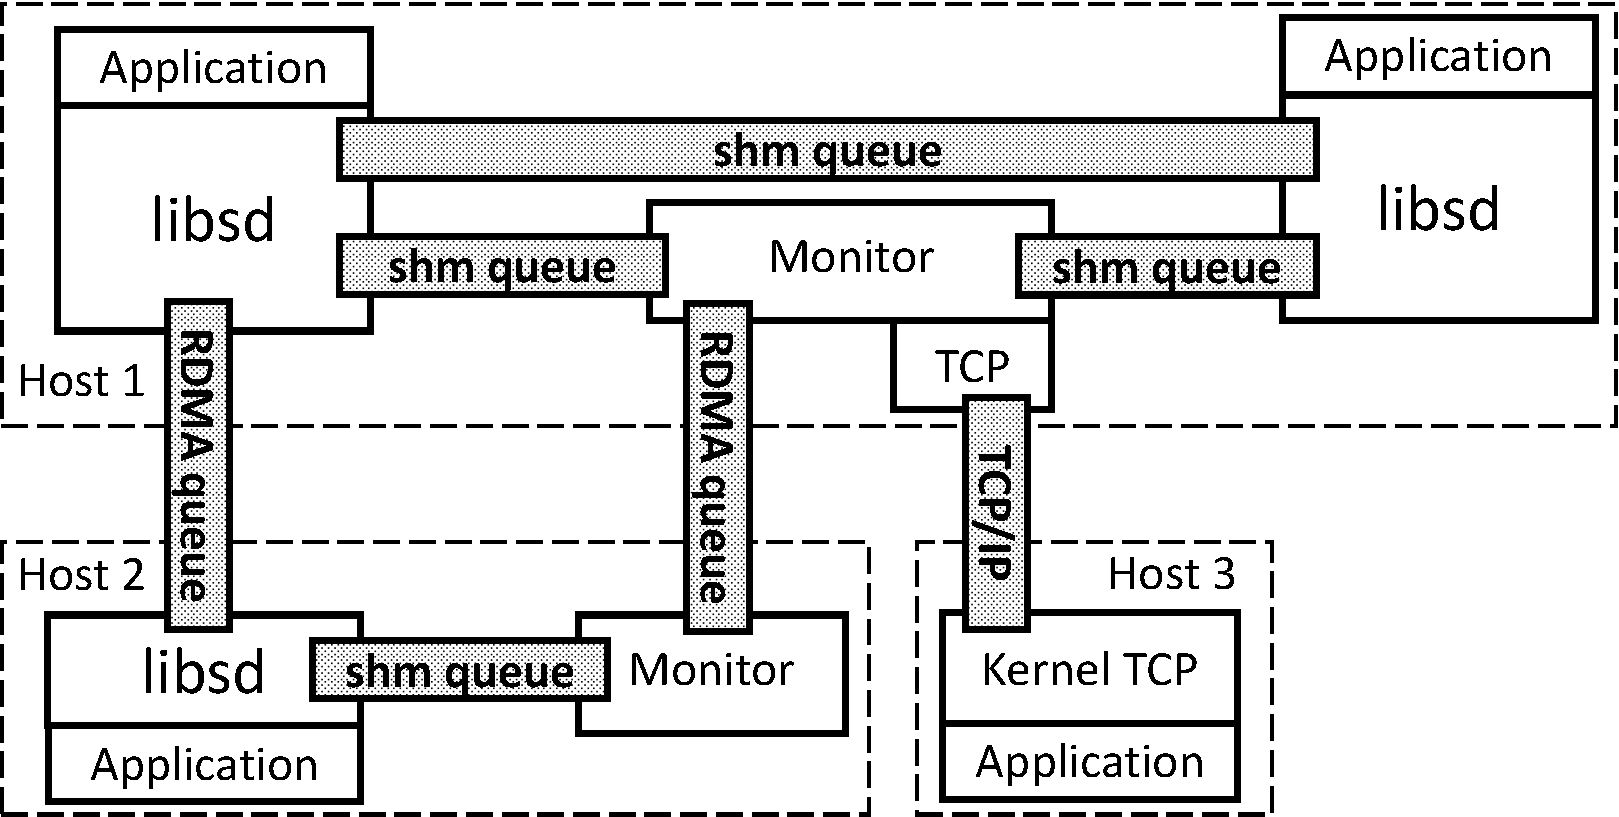
\includegraphics[width=0.8\textwidth]{images/architecture_new}
	
	\caption{\sys {}的体系结构。 主机1和2具有RDMA能力,而主机3不具备RDMA。}
	\label{socksdirect:fig:architecture}
	\vspace{5pt}
\end{figure}


\iffalse
\begin{figure}[htbp]
	\centering
	\subfloat[Traditional queue structure.]{
		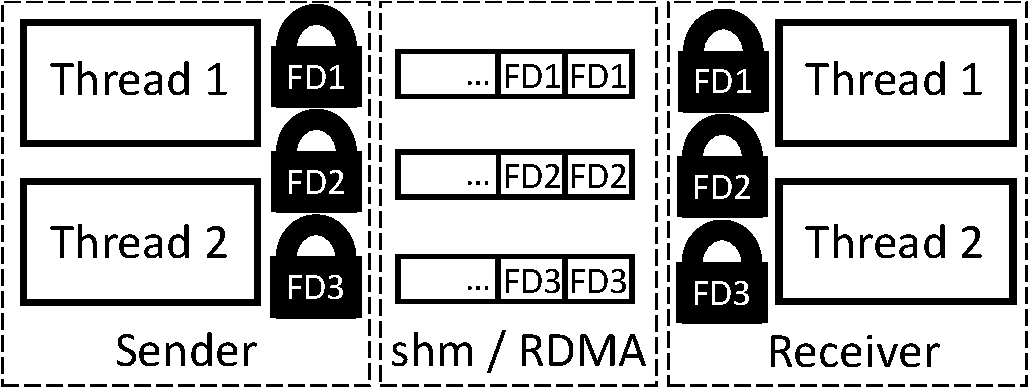
\includegraphics[width=0.4\textwidth]{images/fork_linux}
	}
	
	\subfloat[\sys{} queue structure.]{
		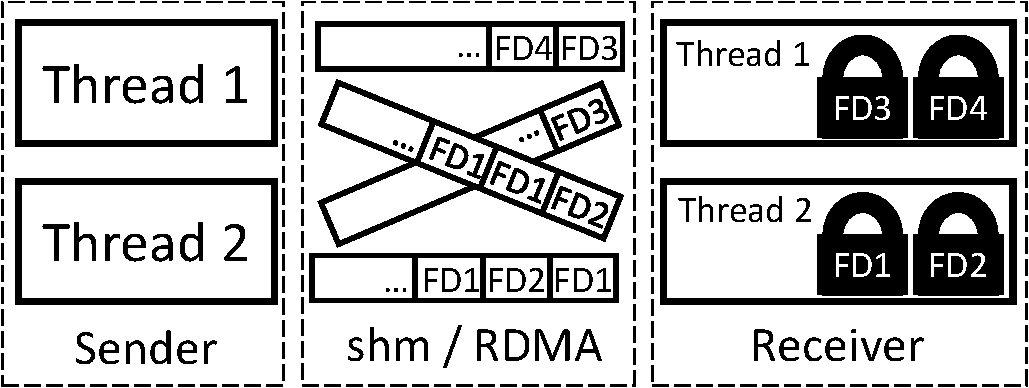
\includegraphics[width=0.4\textwidth]{images/fork_rdwr}
	}
	
	\caption{Comparison of queue structures. Assume sender and receiver each has two threads. First, \sys{} creates peer-to-peer queues between each pair of sender and receiver threads. Rather than protecting the queue with locks, we designate each 文件描述符 to a receiver thread to ensure ordering. Second, data from all connections (文件描述符) are multiplexed through a shared queue, instead of one queue per 文件描述符.}
	\label{socksdirect:fig:fork-rdwr}
\end{figure}
\fi


%As shown in Figure~\ref{socksdirect:fig:architecture}, the core component of \sys{} is a user-space library \libipc{}.

为了简化部署和开发 \cite {andromeda},以及删除内核交叉开销,本章在用户空间而不是内核中实现\sys。
要使用\sys,应用程序通过设置\texttt {LD\_PRELOAD}环境变量来加载用户空间库\libipc {}。 \libipc {}拦截标准C库中与文件描述符(文件描述符)操作相关的所有Linux API。它使用\emph {文件描述符重映射表}来区分套接字文件描述符与内核文件描述符(例如文件和设备),在用户空间中实现套接字功能并将其他功能转发到内核。
从安全的角度来看,因为\libipc {}驻留在应用程序地址空间中,它的行为不可信。例如,如果恶意应用程序在\libipc {}中强制执行,则可能会绕过防火墙策略。此外,TCP端口是一个需要分配的全局资源 \cite {lin2016scalable,nsdi19freeflow}。因此,需要在\libipc {}之外的可信组件来强制实施访问控制和管理全局资源。

为此,本章在每个主机上设计一个\emph {monitor}守护进程来协调控制平面操作,例如连接创建。监视器是系统服务。在每个主机中,所有加载\libipc {}的应用程序必须与主机的监视器守护程序建立共享内存(SHM)队列,从而形成控制平面。在数据平面上,应用程序构建对等队列以直接通信,从而减轻了监视器守护程序的负担。图 \ref {socksdirect:fig:architecture}显示了\sys {}的体系结构。


%To this end, we regard processes as a shared-nothing distributed system that communicates through message passing.
%We design a secure control-plane protocol between applications and the monitor, and a data-plane protocol between applications.

为了实现低延迟和高吞吐量,\sys {}使用SHM进行主机内部和RDMA进行主机间通信。
每个套接字连接都映射到SHM队列或RDMA QP。
SHM或RDMA QP由唯一令牌标记,因此其他非特权进程无法访问它。
套接字发送操作转换为对远程端点上的套接字缓冲区的SHM或RDMA写操作。

对于\emph {intra-host}通信,通信发起者首先向本地监视器发送请求,然后监视器在两个应用程序之间(可能在不同的容器中)建立共享内存队列。 之后这两个应用程序可以直接通信。


%During initialization, \libipc{} connects to the local monitor via a shared memory queue.
%To enforce access control policies and support overlay networks, % and load balance new connections to multiple listeners, 
%connection request is always sent to the local monitor.
%For local peers, the monitor just construct a shared memory queue between the two applications , %so they can communicate directly.

对于\emph {inter-host}通信,两个主机的监视器都参与其中。当应用程序连接到远程主机时,其本地监视器会建立常规TCP连接,并检测远程主机是否支持\sys {}。
如果是这样,它会在两个监视器之间建立一个RDMA队列,以便可以更快地创建两个主机之间的未来连接。远程端的监视器调度与目标的连接,并帮助两个应用程序建立RDMA队列,如图 \ref {socksdirect:fig:architecture}中的主机1和2之间。如果远程主机不支持\sys {},它将继续使用TCP连接,如图 \ref {socksdirect:fig:architecture}中的主机1和3之间。详细的连接管理协议在Sec .~ \ref {socksdirect:subsec:connection-management}中介绍。

为了确保线程安全并避免锁定,以及支持fork和container实时迁移,本章针对只有一对发送和接收线程处于活动状态的常见情况进行了优化,同时确保所有情况下的正确性(Sec .~ \ref {socksdirect:subsec:fork})。
为了消除缓冲区管理开销,设计了一个环形缓冲区,每个主机间消息平摊下来只需要一次RDMA写操作,每个主机内消息需要一个缓存迁移(Sec .~ \ref {socksdirect:subsec:lockless-queue} )。
本章进一步设计了一种零拷贝机制,可以在发送和接收端删除大型消息的数据副本(Sec .~ \ref {socksdirect:subsec:zerocopy})。
最后,Sec .~ \ref {socksdirect:subsec:process-mux}提供了事件通知机制。

%In order to remove synchronization overhead for multi-threaded applications, we treat each thread as a separate process.
%%Although threads in a process share memory, we use thread-specific storage for most states in \libipc{}.
%For two communicating applications, we create peer-to-peer queues between each pair of sender and receiver threads to avoid synchronization cost of contending on the same queue.
%In Sec.~\ref{socksdirect:subsec:fork}, we present the peer-to-peer queue design that preserves FIFO ordering semantics and avoids starvation, especially when a process forks or creates a new thread.
%To maintain performance with many concurrent connections, rather than creating separate queues for each connection, we multiplex data from all connections through one queue.
%In Sec.~\ref{socksdirect:subsec:multiplex-conn}, we present the design of multiplexed queue that avoids head-of-line blocking and supports fetching data from any multiplexed connections.

%Inspired by Unikernels~\cite{madhavapeddy2013unikernels}, we move networking and IPC functions from the kernel to user space. Similar to existing works~\cite{peter2016arrakis,jeong2014mtcp,libvma}, we leverage multiple queues in modern 网卡s to enable user-space direct access to network. %The kernel is still responsible for process creation, scheduling, virtual memory and device management, but no longer on the critical path of performance.
%To maintain compatibility with existing Linux applications, we design a user-mode library \libipc as a drop-in replacement of the system call wrappers in the GNU C library (glibc). \libipc{} implements network socket functions in user mode, and adds a wrapper to other system calls to track process creation and memory allocation. \libipc{} is not considered a secure domain, as it shares memory space with the application. When \libipc{} is loaded, it creates a Linux native \textit{bootstrap socket} to the \textit{monitor} daemon, then creates a shared memory queue to the monitor.

%Even though multiple threads in the same process share memory space, we still treat each thread as a separated process and use thread-specific storage to store states in \libipc. In the following text, unless explicitly mentioned, we use a ``process'' to refer to a regular process or a thread.

\section{设计}
\label{socksdirect:sec:design}


\subsection{无锁套接字共享}
\label{socksdirect:subsec:fork}


\begin{figure}[htbp]
	\centering
	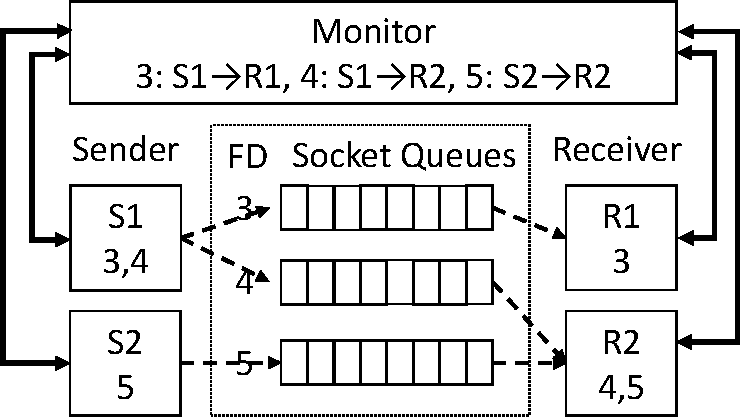
\includegraphics[width=0.6\textwidth]{images/queue_arch}
	
	\caption{无锁套接字与两个发送器和两个接收器线程共享。 虚线箭头表示每个套接字的活动发送方和接收方。 每个线程跟踪其活动套接字并通过独占队列与监视器通信。}
	\label{socksdirect:fig:queue-arch}
\end{figure}

大多数套接字系统都获得了一个per-文件描述符锁,以使线程和进程共享套接字(Sec .~ \ref {socksdirect:subsec:per-operation-overhead})。
以前的工作 \cite {boyd2010analysis,clements2015scalable}表明许多套接字操作不可交换,并且不能始终避免同步。
本章利用SHM消息传递比锁定 \cite {roghanchi2017ffwd}便宜得多的事实,并使用消息传递作为独占同步机制。

逻辑上,套接字由两个相反方向的FIFO \emph {queues}组成,每个FIFO具有多个并发发送器和接收器。
本章的目标是在保持FIFO语义的同时最大化通用情况性能。
我们提出两点观察:首先,由于成本高,在高性能应用程序中创建fork和线程很少。
其次,几个进程从共享套接字发送或接收并不常见,因为套接字的字节流语义使得很难避免接收部分消息。
%如果应用程序需要同时发送或接收,则通常使用消息代理 \cite {hintjens2013zeromq,rabbitmq2017rabbitmq,kreps2011kafka}。
常见的情况是应用程序隐式地将套接字从一个进程迁移到另一个进程,例如将事务从master卸载到工作进程。

\iffalse
Based on the observations, we propose the following requirements:

\begin{enumerate}[noitemsep,nolistsep]
 \item \textbf{Synchronization-free.} With multiple senders and receivers, if only one pair of sender and receiver is active, no synchronization should occur.
 \item \textbf{Multi-sender scalability.} Multiple processes may send data concurrently through a shared socket. With multiple active senders and a single receiver, if the receiver is not a bottleneck, the throughput should scale.
 \item \textbf{Self-stabilization.} Certain operations (\textit{e.g.} \texttt{fork}) may slow down the system temporarily, but after that the performance should converge back to normal.
\end{enumerate}

For compatibility with Linux semantics, we also need to ensure message ordering and liveness:
\begin{enumerate}[noitemsep,nolistsep]
\item \textbf{Single receiver ordering.} For a specific pair of sender and receiver, the received messages have the same ordering as they were sent.
\item \textbf{Multiple receiver ordering.} The order of \texttt{send} and \texttt{recv} operations for one sender and multiple receivers should be linearizable. If receiver $R_1$ receives $D_1$ before receiver $R_2$ calls \texttt{recv} and gets $D_2$, we guarantee that $D_1$ is sent before $D_2$.
\item \textbf{Deadlock-free.} If a socket buffer is not empty when \texttt{recv} is called by one or more receivers, at least one receiver should get data.
\item \textbf{Starvation-free.} If a sender keeps sending, any receiver trying to \texttt{recv} will eventually get some data.
\end{enumerate}
\fi

本章的解决方案是每个\emph {套接字队列}(套接字的一个方向)有\emph {send token}和\emph {receive token}。
每个令牌都由\emph {active thread}持有,它具有发送或接收的权限。
因此,在任何时间点只有一个活动的发送方线程和一个活动的接收方线程。
套接字队列在线程和进程之间共享,允许来自一个发送方和一个接收方的无锁访问(详细信息将在Sec .~ \ref {socksdirect:subsec:lockless-queue}中讨论)。
当另一个线程想要发送或接收时,它应该请求\emph {接管}令牌。

%\RED{Need performance comparison in a figure.}

每种类型的操作的详细信息如下:a)数据传输(\texttt {send}和\texttt {recv}),b)添加新的发送者和接收者(\texttt {fork}和线程创建 ),c)容器实时迁移,和d)连接关闭。

\subsubsection{发送/接收操作}
\label{socksdirect:subsubsec:fork_rdwr}


当一个线程没有发送令牌但想要通过套接字发送时,非活动线程需要\emph {接管}令牌。
如果在非活动线程和活动线程之间创建直接通信通道,则会有对等队列,其数量为线程数的二次方,或者是具有锁定的共享队列。
为了避免这两种开销,在\emph {接管}过程中使用监控守护进程作为代理。
此消息传递设计还具有以下优点:发送方进程可以位于不同的主机上,这在容器实时迁移中非常有用。

接管过程如下:
非活动发送方向监视器发送\emph {take over}命令,监视器将其添加到等待列表并将命令代理到活动发送方。
当活动发送方收到请求时,它会将发送令牌发送给监视器。
监视器将令牌授予等待列表中的第一个非活动发送者,并更新活动发件人。
非活动发件人可以在收到令牌后发送。
此机制无死锁,因为至少有一个发送方或监视器持有发送令牌。
它也是无饥饿的,因为每个发送者最多可以出现在等待列表中一次,并按FIFO顺序提供。

接收器侧的接管过程类似。


%\begin{figure}[t]
%	\centering
%	
\includegraphics[width=0.3\textwidth]{images/fixme}
%	\caption{This figure shows a stable connection handled by multiple senders and receivers.}
%	\label{socksdirect:fig:fork-bipartitegraph}
%\end{figure}

\subsubsection{Fork,Exec 和线程创建}
\label{socksdirect:subsubsec:fork_fork}


\iffalse
\begin{figure}[t]
	\centering
	\subfloat[Traditional locking]{
		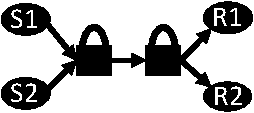
\includegraphics[width=0.15\textwidth]{images/one_conn3}
		\label{socksdirect:fig:fork-locking}
	}
	\hspace{0.02\textwidth}
	\subfloat[SocksDirect peer-to-peer]{
		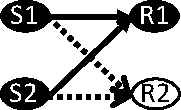
\includegraphics[width=0.11\textwidth]{images/one_conn1}
		\label{socksdirect:fig:fork-p2p}
	}
	\hspace{0.02\textwidth}
	\subfloat[S2 forks to S2' and S3]{
		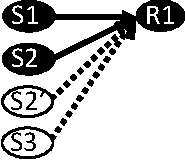
\includegraphics[width=0.1\textwidth]{images/one_conn2}
		\label{socksdirect:fig:fork-fork}
	}
	
	\caption{Inter-process queue architectures for a shared socket. Dashed arrows represent non-activated queues.}
\end{figure}
\fi

\begin{figure}[htbp]
	\centering
	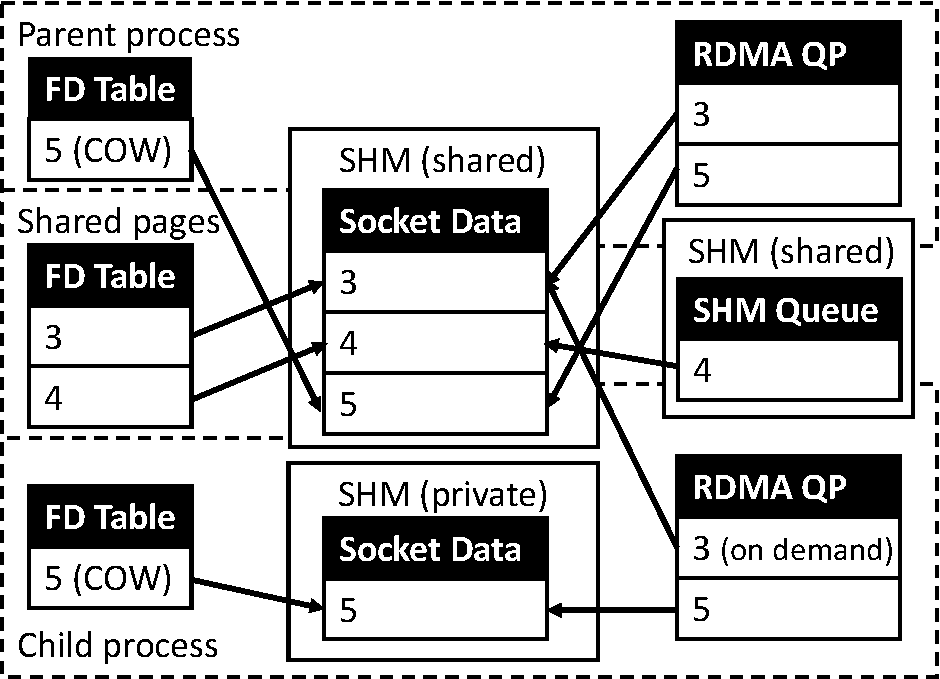
\includegraphics[width=0.6\textwidth]{images/fork_memory}
	
	\caption{fork后的内存布局。 文件描述符 3和4在fork之前创建并因此共享。 在fork之后,父进程和子进程分别创建一个新的文件描述符 5,它在文件描述符表中写入时被复制。 文件描述符 3和4的套接字元数据和缓冲区在SHM中并因此被共享。 子进程创建一个新的SHM来存储文件描述符 5的套接字元数据和缓冲区,当它再次分叉时,它将与子进程共享。 RDMA QP位于私有内存中,而SHM队列是共享的。}
	\label{socksdirect:fig:fork-memory}
\end{figure}
\textbf {套接字数据共享。}
主要的挑战是在\texttt {fork}和\texttt {exec}之后共享套接字元数据,缓冲区和底层传输。
内存空间在fork之后变为写时复制并在exec之后被擦除,但是套接字文件描述符仍应该可用。
我们使用共享内存(SHM)来存储套接字元数据和缓冲区,因此在fork之后,数据仍然是共享的。
要在exec之后附加SHM,\libipc {}将连接到监视器以获取其父进程的SHM密钥。
在fork之后,因为父进程看不到子进程创建的套接字,所以子进程创建一个新的SHM来存储新套接字的元数据和缓冲区。

现在需要共享连接到对等端的底层传输。
SHM传输不需要特别小心,因为fork / exec之前创建的SHM仍然在fork / exec之后共享。
但是,RDMA与fork / exec有问题,因为DMA内存区域不在SHM中。
它们在fork之后变为写时复制,而网卡仍然从原始物理页面DMA,因此子进程不能使用现有的RDMA资源。
在exec之后,整个RDMA上下文被清除。
本章的解决方案是让子进程在fork / exec之后重新初始化RDMA资源(PD,MR等)。
当子进程使用在fork之前创建的套接字时,它会要求监视器与远程端点重新建立RDMA QP。
因此,远程可能会看到一个套接字的两个或更多QP,但它们链接到套接字元数据和缓冲区的唯一副本。
图 \ref {socksdirect:fig:fork-memory}显示了一个fork示例。

\textbf {文件描述符 space sharing。}
与套接字数据不同,文件描述符空间在fork之后变为写入时复制:现有文件描述符是共享的,但新文件描述符由creater进程专有。
所以文件描述符重映射表驻留在堆内存中,这是fork之后的copy-on-write。
要在exec之后恢复文件描述符重映射表,它将在exec之前复制到共享内存,并在\libipc {}初始化期间附加到新进程。

\textbf{安全。}
安全性是一个问题,因为恶意进程可能将自己伪装成特权父进程的子进程。
要在监视器中标识父关系和子关系,当应用程序调用\texttt {fork},\texttt {clone}或\texttt {pthread\_create}时,\libipc {}首先生成一个用于配对的秘密并将其发送到监视器,然后调用\emph {libc}中的原始函数。
在fork之后,子进程为监视器创建一个新的SHM队列并发送秘密(子进程继承父内存空间并知道该秘密)。
因此,监视器可以将子进程与父进程配对。

\textbf {监视行动。}
在fork,exec或线程创建时,每个现有套接字需要将发送方添加到发送方向,将接收方添加到接收方向。
父进程继承该令牌,因此子进程始终处于非活动状态。

%The socket queues are in SHM between parent and child processes.
%However, to avoid synchronization in accessing shared metadata, the metadata is in thread local storage and copied from parent to child.
%To maintain isolation between parent and child, monitor creates new shared memory queues to replace all queues in \emph{both} parent and child, as Figure~\ref{socksdirect:fig:fork-fork} shows. We do not reuse queues due to potential isolation violation. %The monitor then sends credentials of new queues to parent and child via bootstrap sockets. 
%Each peer process is notified of the new queues and the new process. From then on, parent and child processes have isolated queues to the monitor and peers.

%A harder challenge comes from socket connection sharing between parent and child processes.
%A major challenge is how to handle the remaining data in the original send and receive queues.

%For each unidirectional queue, we discuss the behavior of related processes in four cases:
%\begin{enumerate}
%	\item A sender process itself forks.
%	\item A receiver of a sender process forks.
%	\item A receiver process itself forks.
%	\item A sender of a receiver process forks.
%\end{enumerate}

%The general process of fork is that after monitor is notified of the fork, it creates shared memory between the newly created process and all the processes which previously have connections with the parent process. The key challenge lies in the fork is that how to deal with the existing data in the connection to guarantee the order requirements.

%\textbf{Receiver fork.}
%First we look at a simple case when a receiver forks. Recall that only one receiver has exclusive access to a socket, as stated in Sec.~\ref{socksdirect:subsubsec:fork_rdwr}. The parent process inherits receive permission. When a sender receives fork notification of its peer, it copies all data from original queues to new queues of the parent process.

%\textbf{Sender fork.}
%When a sender forks, things are more complicated. We need to guarantee that all data sent prior to \texttt{fork} is consumed before the data sent after \texttt{fork}.

%Our solution is to let receivers drain the original queue first before switching to the new queues. After \texttt{fork}, both parent and child send data to its new queue. When the receiver is notified of the fork, it keeps track of the original queue and consumes all data in it before activating new queues. Note that the parent or child may fork again before the original queue is drained. With this in mind, the receiver maintains a forest data structure to track dependency of queues. The root of each tree in the forest is the oldest queue to receive from. Each non-leaf node has two children indicating the new queue of parent and child processes. If a non-leaf root queue becomes empty, it will be removed, and the two children queues will be promoted to root nodes.

%\textbf{Takeover During Fork.}
%After a sender forks, the receivers still need the takeover mechanism to arbitrate remaining messages in the original queue. However, both parent and child senders have dropped the original queue and will not respond to takeover requests. A similar situation occurs when a sender process dies. Our solution is to let the receivers use atomic operations to compete for remaining data in the original queue. Since this case rarely happens, the performance of the overall design is not affected.

%Things become much more complicated when cases 1,4 happens after cases 2,3 happening. After receiver forks, the unique sender is responsible for receiving ``takeover message'' and resend the data to new receivers. However, if sender forks following the receiver forks, according to the methods we mentioned above, there is no sender responsible for processing ``takeover message''. Our solution is that we require the receivers to poll the data from the old shared memory queue and compete for data. Since this case rarely happens, the performance of the overall design is not affected.

\subsubsection{容器热迁移}
\label{socksdirect:subsubsec:container_live_migration}


\textbf {在套接字队列中迁移剩余数据。}
由于\libipc {}在与应用程序相同的进程中运行,因此其内存状态将与应用程序一起迁移到新主机。
内存状态包括套接字队列,因此不会丢失正在传输(已发送但未接收)的数据。
套接字只能在容器内共享,并且容器中的所有进程都会一起迁移,因此迁移后可以取消分配原始主机上的内存。

\textbf {监控状态的迁移。}
监视器跟踪侦听套接字信息,活动线程和每个连接的等待列表以及共享内存机密。
在迁移期间,旧监视器会转储已迁移容器的状态并将它们发送到新监视器。

\textbf {建立新的沟通渠道。}
迁移后,所有通信通道都已过时,因为共享内存在主机上是本地的,而RDMA不支持实时迁移 \cite{nsdi19freeflow,slim}。
首先,新主机上的迁移容器需要与本地监视器建立连接。
本地监视器指示以下过程。
两个容器之间的主机内连接可能变为主机间,因此\libipc {}在这种情况下创建RDMA连接。
两个容器之间的主机间连接可能成为主机内部,\libipc {}创建共享内存连接。
最后,\libipc {}重新建立剩余的主机间RDMA和主机内共享内存连接。


%\subsubsection{Connection Creation}
%\label{socksdirect:subsubsec:fork_new}
%

%A connection created by a thread can be accessed by all threads in the same process.
%To avoid creating redundant queues and connection states, \libipc does not share the 文件描述符 eagerly with other threads, because most threads in existing applications do not use connections created by other threads.
%When a thread do want to accesses a 文件描述符 that belongs to another thread, \libipc sends a message to the owner thread and requests sharing the 文件描述符. %This procedure is exactly the same as sharing existing connections during thread creation (Sec.~\ref{socksdirect:subsubsec:fork_fork}). %The sharing procedure only happens once for every connection and thread. Sharing existing connections eagerly during thread creation is an optimization. First, children threads are more likely to use existing connections than siblings. Second, batch processing improves performance.

%\subsubsection{Connection Close}
%\label{socksdirect:subsubsec:fork_close}
%

%Close is the operation that all of the processes leave the connection. The synchronization is  especially challenging since all the processes are run in parallel. One challenge lies in file descriptors are managed by decentralized processes and are possibly reused. One process close a connection while the others are doing compute intensive tasks is a case. It is possible that the file descriptor of the old process is reused and a new connection is setup with the same file descriptor. The other process may notice the close of the old connection and also call close on its own side, which lead to the new connection setup by the previous process closed due to the match of same file descriptor. 

%To satisfy the synchronization requirements, the close function call is all completed by message passing. The caller of close need to wait for ACK from all the other peers before release resources. i.e. the status of the connection.

%\textbf{Broadcast.}
%When a process calls \texttt{close}, all its peers cannot send to or receive from the 文件描述符. In this sense, 
%A socket is closed if all shared processes close it. So, we need to multicast a notification to the peers and collect responses from them. A challenge arises when \texttt{close} is interleaved with \texttt{fork}. Since \texttt{fork} and \texttt{close} do not commute~\cite{clements2015scalable}, we need a rule to determine their partial order. We make the choice that the ordering is determined by the initiator of \texttt{close}. If a process calls \texttt{close} before receiving fork notification, it will piggyback close notification with fork completion to both parent and child processes.

%\textbf{Handshake before releasing resource.}
%Another challenge is caused by 文件描述符 reuse after close. As stated in Sec.~\ref{socksdirect:subsec:socket-api}, a 文件描述符 is deleted after receiving shutdown message of both directions. With multiple processes sharing a connection, after one process calls \texttt{close}, others can still use the connection. Consequently, a process deletes a 文件描述符 only after receiving shutdown messages of both directions from all peers of the 文件描述符.

%Another challenge lies in the close of a connection is that close is a broadcast operation while send/receive is sent to a specific process. Besides, fork and close are immutable operations while the scalability requirements of the system impose the constraint that all the operations run asynchronously. As a result, a rule to determine the partial order is required.

%In \libipc, we make the choice that the order of fork and close is determined at the start point of the fork operation and the end point (after receiving all the ACKs). By making this choice, when a process waiting fork close ACK encounters fork message, it could send a separate close request to newly created process, which guarantees all the processes closed.

\iffalse
\subsection{Multiplex Sockets via One Queue}
\label{socksdirect:subsec:multiplex-conn}

\begin{figure}[t]
	\centering
	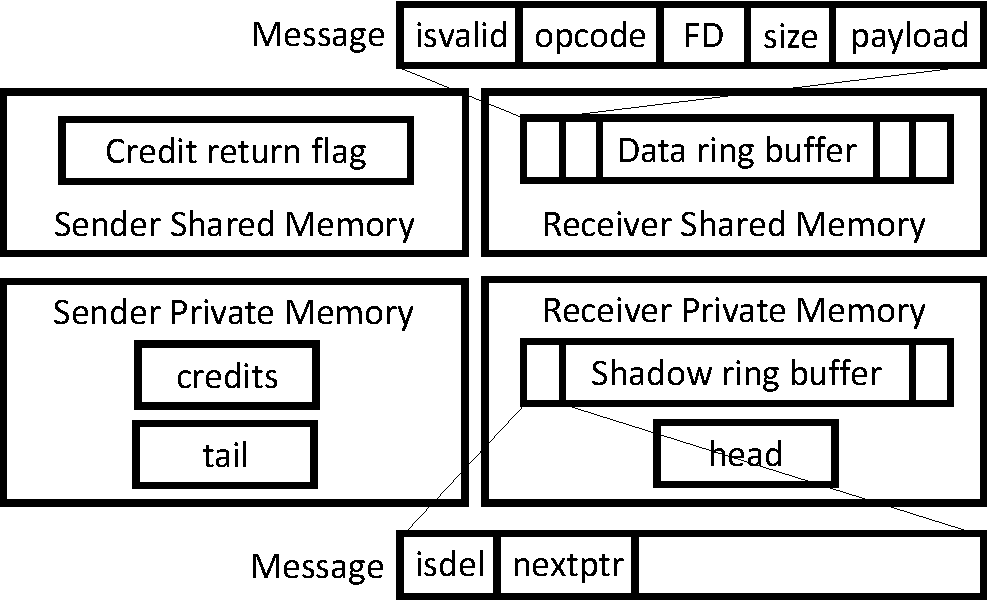
\includegraphics[width=0.4\textwidth]{images/locklessq_new}
	
	\caption{The structure of an inter-process queue.}
	
	\label{socksdirect:fig:locklessq-structure}
\end{figure}


%\textbf{Multiplex connections in event-driven applications.}
To reduce memory footprint and improve locality of memory accesses, we use one queue to multiplex all connections between a pair of threads. Each data item in the queue is marked with its 文件描述符. By using a single queue, we reduce per-socket memory footprint, random memory accesses and cache misses.

\textbf{Message format.}
As shown in Figure~\ref{socksdirect:fig:locklessq-structure}, the main component of the queue is a \emph{data ring buffer}, where messages are stored back-to-back.
Each message in the ring buffer consists of an 8-byte header and a variably sized payload. The header consists of an \textit{isvalid} flag, an opcode, the receiver's 文件描述符 number and the payload size. Messages are aligned to 8 bytes to ensure header write atomicity.% and accelerate payload copy.

\textbf{Event polling.}
We maintain a bitmap of each epoll 文件描述符 set.
When \texttt{epoll\_wait} is called, we scan all data queues round-robin and check the 文件描述符 of each data message against the bitmap. If the 文件描述符 is in the bitmap, an event is returned to the application.
A global cursor exists to resume data queue scanning from the last position in the last scanned queue.

A per-queue cursor records the last scanned position in each queue to avoid scanning a message multiple times.
To speedup repeated receive operations of a specific 文件描述符, we build a linked list of messages for each 文件描述符 as a side product of event polling.
Each 文件描述符 maintains positions of the first and last scanned but unread messages of the 文件描述符.
When a new message of the 文件描述符 is scanned, the \emph{nextptr} pointer in the last message is updated to point to the new message.

To poll events from sockets and other 文件描述符 (handled by kernel) at the same time, \libipc{} creates an \textit{epoll thread} in each process to wait on all 文件描述符 handled by kernel. When it receives a kernel event, it broadcasts the event to application threads via shared memory queues. %\texttt{Epoll\_wait} in \libipc{} will return such kernel events in addition to socket events. %Note that Linux allows an event to be received by multiple threads sharing the 文件描述符.

\textbf{Pick from middle of queue.}
In order to support receiving data from a specific 文件描述符, the queue needs to support picking a message in the middle with a specific 文件描述符.
Fortunately, this does not happen frequently. Event-driven applications typically process incoming events in a FIFO order. For \texttt{epoll\_wait} in level trigger mode, we iterate through all messages in the queue and return those in the set of registered 文件描述符. When applications call \texttt{recv}, \libipc{} would usually dequeue the message at head.

To pick from middle of queue, receiver traverses messages in the ring buffer. During traversal, receiver iterates messages from \textit{head} until free space in ring buffer, determined by \textit{isvalid}. Hence, receiver cannot clear \textit{isvalid} when a non-head message is dequeued. That's why each message has an \textit{isdel} flag. When a message is dequeued from the middle, its \textit{isdel} is set. %If the message at \textit{head} has \textit{isdel} set, the receiver advances \textit{head} and repeats this step.

\textbf{Head-of-line blocking.}
%Second, if application does not receive from a 文件描述符 for a long time, data items of the 文件描述符 may fill up the queue and starve other 文件描述符.
If application does not receive from a 文件描述符 for a long time, the empty space in queue will become fragmented.
When data queue is full, the sender sends a message via emergency queue to trigger garbage collection in the receiver.
The receiver scans empty space in the middle of queue and moves remaining messages, so that empty space can be returned to the sender.
%To avoid starvation, we need at least one byte of headroom per 文件描述符. Accordingly, we design a single byte \textit{headroom slot} per 文件描述符. When data queue is full and the per-文件描述符 headroom slot is free, sender uses it and sends a notification via emergency queue. Receiver receives from data queue first, then from the headroom slot if it received a notification.

\textbf{Emergency queue.}
Control messages may need to be delivered out-of-band when the queue is full. For example, in order to close the receive direction while sending data, the shutdown message should not be blocked by unconsumed data in the queue. To this end, we add an \textit{emergency queue} alongside each data queue.
A receiver will always retrieve messages in the emergency queue immediately.
\fi

